%%% -*-LaTeX-*-

\chapter{SweetPea Overview}

The previous chapter motivated the need for a software system that facilitates creating replicable, statistically robust experimental designs; this chapter provides a high-level overview of how SweetPea addresses this need.

SweetPea consists of a high-level language and a low-level runtime. The language provides primitives that closely match the terms that scientists use to describe their experimental designs. The runtime synthesizes an experimental sequence which is guaranteed to not prefer any valid solution over any other. The runtime provides this guarantee by representing the experiment as a boolean formula and interfacing with a SAT sampler; this constrains the language to be amenable to being translated into a boolean formula.

In this chapter we'll start by looking at a simple version of a classic psychology experiment, the Stroop test, to identify the fundamental components of an experimental design. Then we'll see how these components are represented in the language and the runtime.

\section{Running Example: the Stroop Experiment}

The Stroop experiment is a well-known psychology experiment, originally published by John Stroop in 1935. A subject is shown a stimulus, and asked to perform a task based on some property of the stimulus; the researcher measures how the subject's reaction time varies depending on the stimulus. One version of this experiemnt involves showing subjects a word printed on a slide and asking them to say the color of the word. All of the words are the names of colors, such as the text 'red' and 'blue'. Some of the stimuli are congruent, meaning that the color of the ink matches the text, such as the word red printed in red ink. Other stimuli are incongruent, such as the word red printed in blue ink (figure \figref{stroop_example}). The Stroop effect is the observation that subjects have a longer reaction time when the stimulus is incongruent.

Let's consider the smallest version of the Stroop experiment, where the stimuli consist of two colors. Each stimulus is specified by independent and control variables, called \emph{factors}: ink color and text. Each factor has two \emph{levels}, red and blue. Figure \figref{simple_full_crossing} shows the \emph{full crossing} of these factors for this simple case, for a total of 4 possible stimuli. For reference, real experiments have on the order of 5 to 8 factors with 2 to 4 levels, leading to tens to hundreds of possible stimuli. The \emph{design} of the experiment is the list of all factors that describe each stimulus. The design of the experiment may contain factors that are not present in the full-crossing.

Each subject is shown an ordering of the possible stimuli. The researchers may want to place additional \emph{constraints} on the ordering, such as first familiarizing the subject with the task by showing some number of congruent stimuli before showing them a mix of congruent and incongruent stimuli. For our small example, let's consider the constraint that there should be no repetitions of stimuli whose text is the same. The ordering in \figref{simple_full_crossing} is a valid ordering which satisifies these constraints, but swapping the order of the first and second trial would produce an invalid ordering under those constraints.

To prove that we do not introduce bias because of the way we construct experimental sequences, we would like to ensure that each valid sequence is equally likely. In this example, we have four stimuli so there are 4 factorial = 24 possible orderings. Of those 24 orderings, 8 satisfy the constraints as shown in \figref{valid_seqs}, and to provide this guarantee we want each of those 8 to be equally likely.


\begin{figure}[t]%
    \centering
    \subfloat[A congruent Stroop stimulus.]{{
\includegraphics[width=7cm]{fig_red_in_red} }}%
  %  \qquad
    \subfloat[An incongruent Stroop stimulus.]{{
\includegraphics[width=7cm]{fig_red_in_blue} }}%
    \caption{Example Stroop stimuli.}%
    \label{fig:stroop_example}%
\end{figure}


\begin{figure}[t]%
    \centering
    \subfloat[The full crossing of possible stimuli.]{{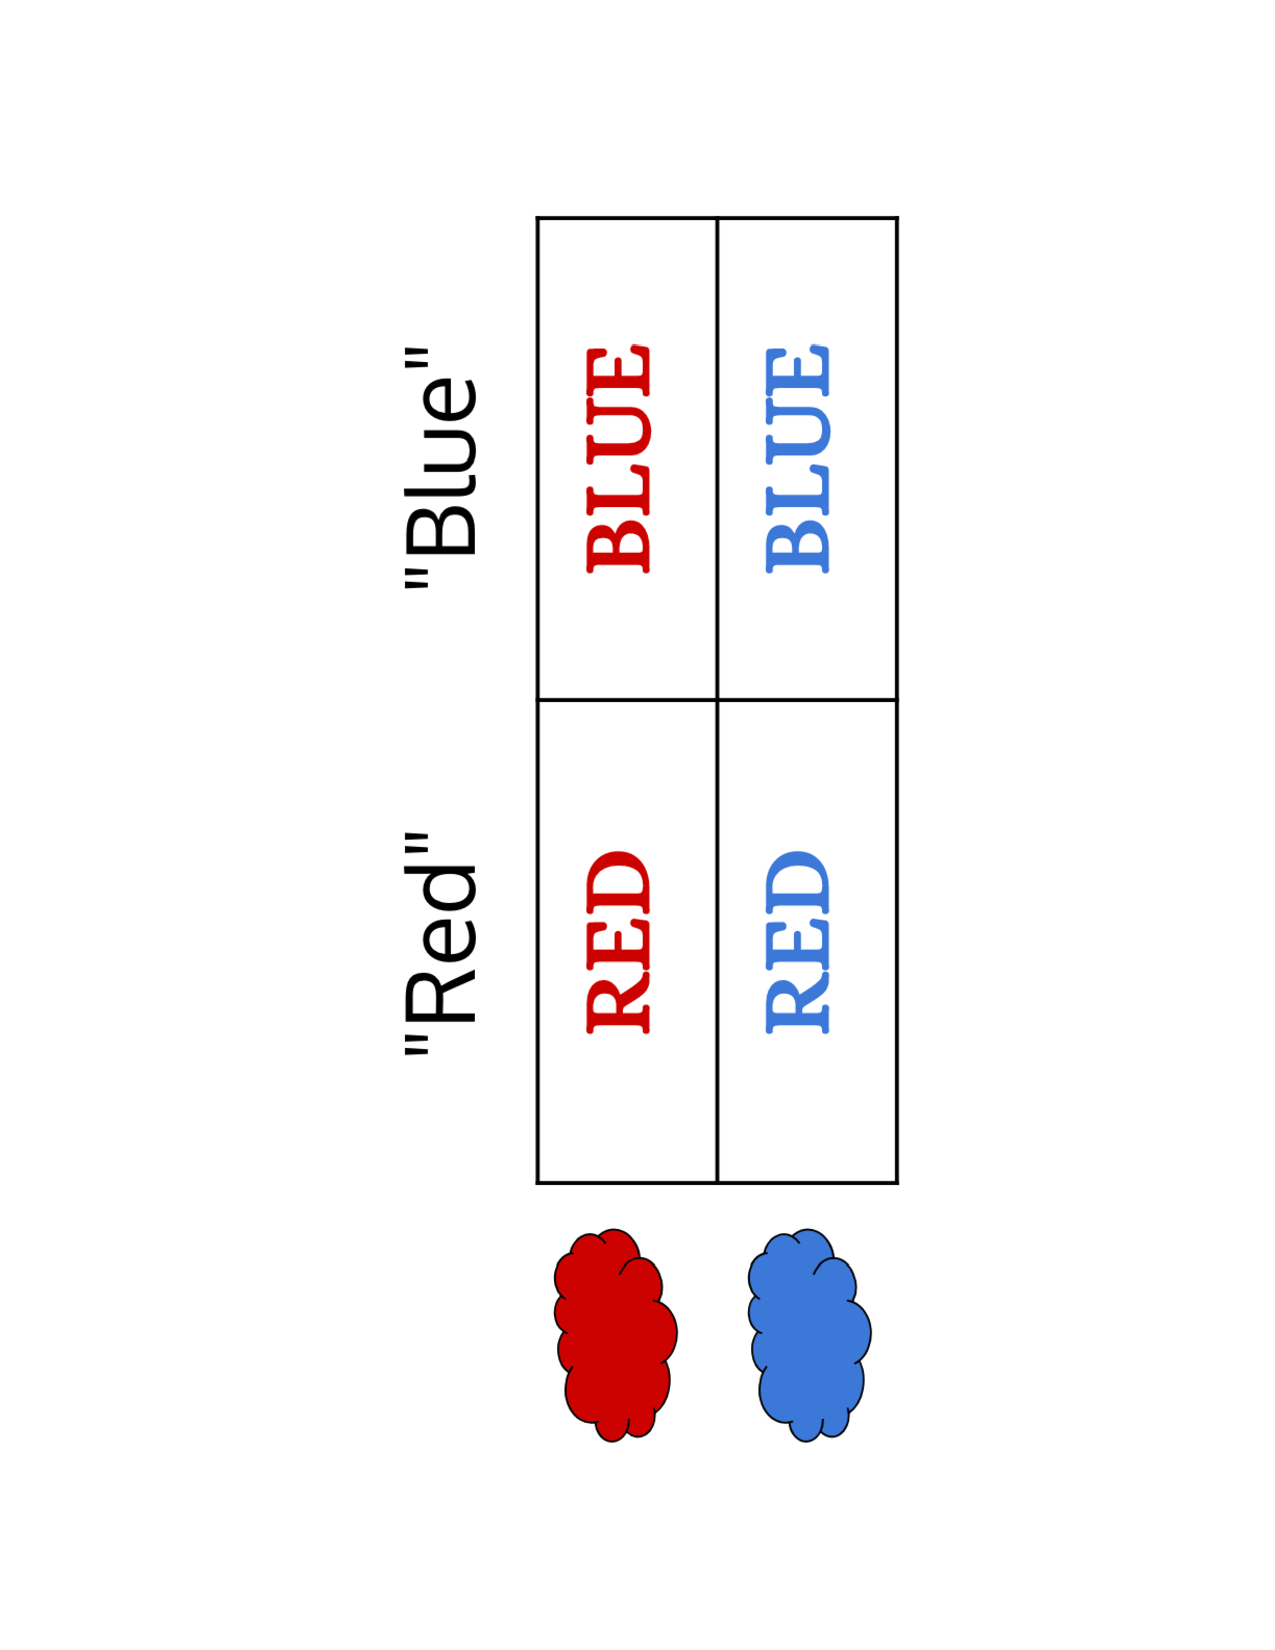
\includegraphics[angle=270,origin=c,width=8cm]{fig_simple_full_crossing}}}%
  %  \qquad
    \subfloat[A possible ordering of stimuli.]{{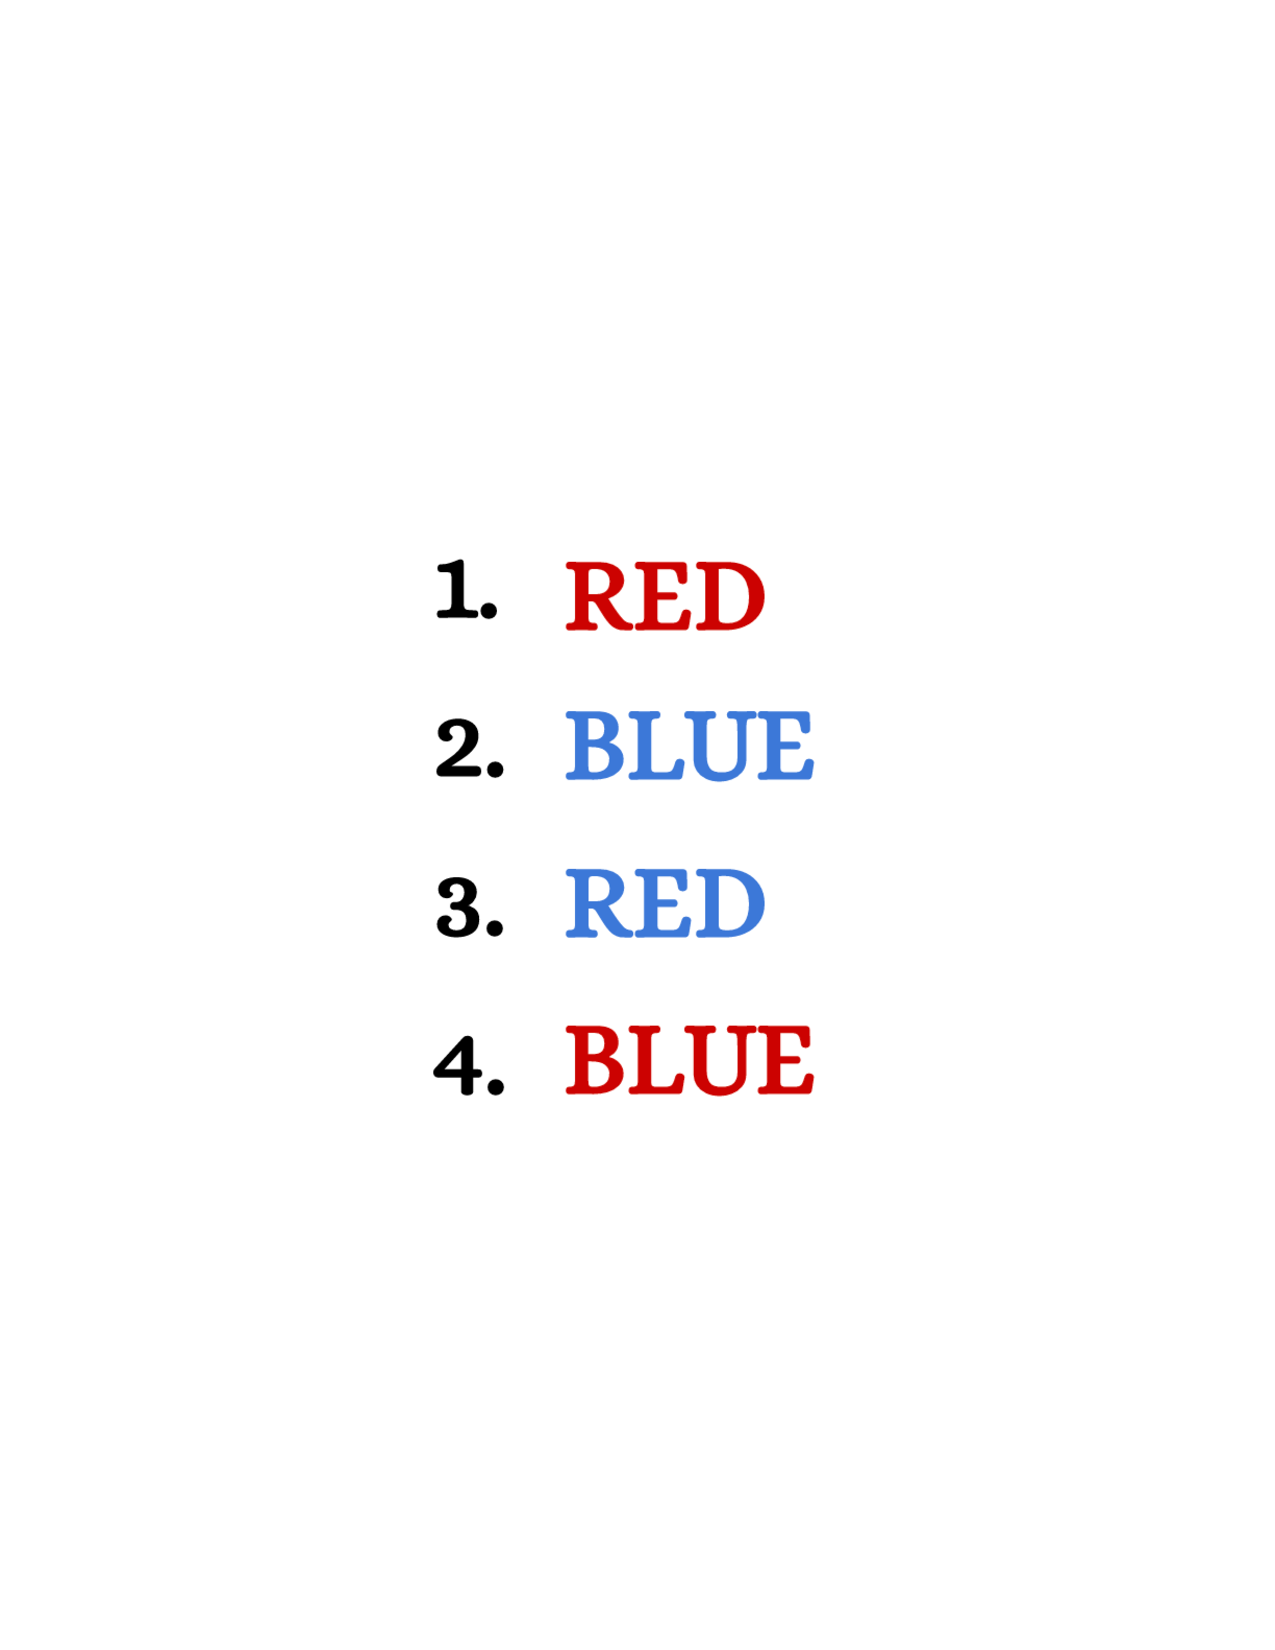
\includegraphics[width=7cm]{fig_possible_ord} }}%
    \caption{All stimuli and a possible ordering.}%
    \label{fig:simple_full_crossing}%
\end{figure}



\begin{figure}[t]
    \centerline{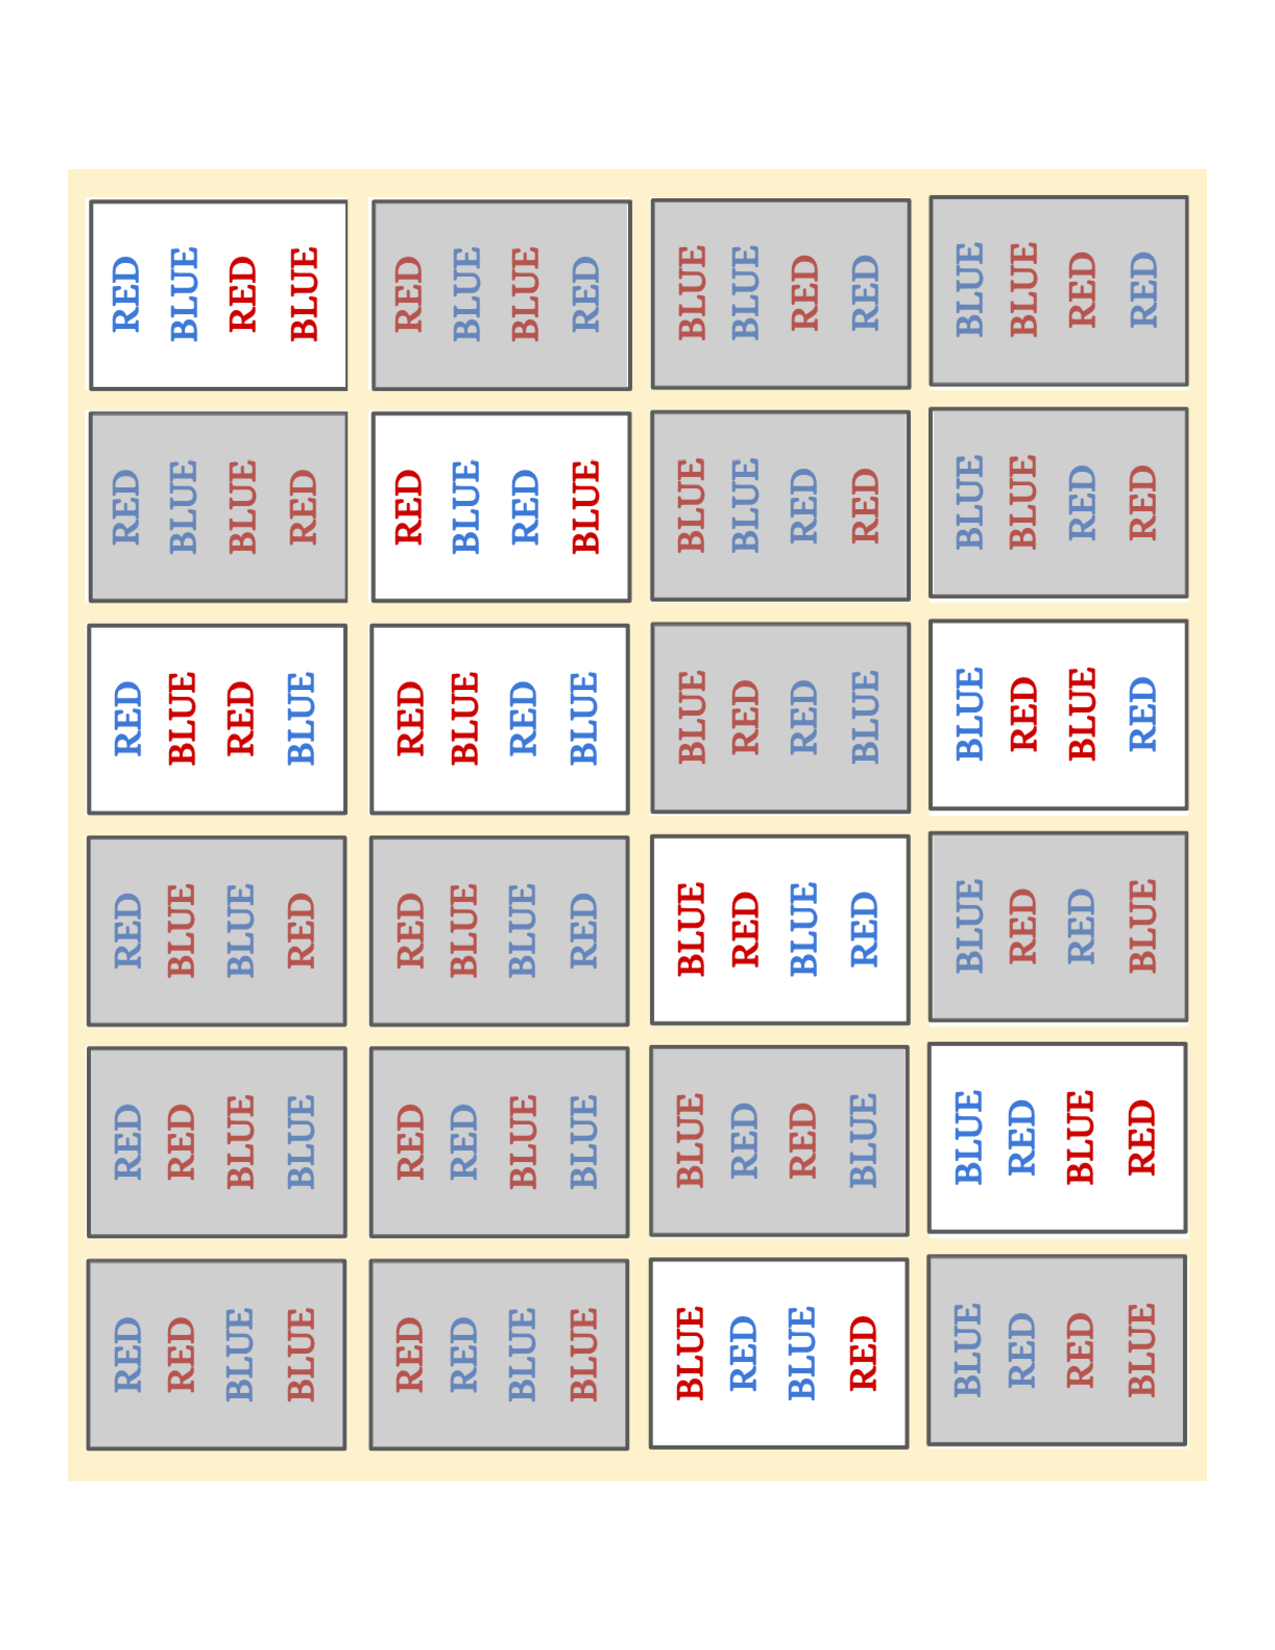
\includegraphics[angle=270,origin=c,width=10cm]{fig_valid_seqs}}
    \caption{Of the 24 possible orderings, the highlighted 8 satisfy the constraints.}%
    \label{fig:valid_seqs}%
\end{figure}


\section{A Language for Experimental Design}

Let's see how the simple Stroop experiment can be represented in SweetPea, and then at how that representation can be translated to a boolean formula to generate an experimental sequence.

The version of the SweetPea language we'll discuss is embedded in Python, so uses Python syntax.

First, we represent the factors directly as a list of levels:

\begin{lstlisting}
ink_color = ("ink_color", ["red", "blue"])
text      = ("text",      ["red", "blue"])
\end{lstlisting}

Next, let's represent the constraint that there should be no repetitions of stimuli whose text is the same:

\begin{lstlisting}
def no_text_reps(text0, text1):
    return text0 != text1

constraints = enforce(Transition(no_text_reps, [text, text]))
\end{lstlisting}

TODO mention ENFORCE

- briefly mention the other parts of experiments: design, crossings, blocks

- the purpose of the language is make it easy to represent experimental designs, while also being amenable to being translated into SAT


\section{A Runtime for Uniform Sampling}

SweetPea can be viewed as a domain-specific interface to SAT-sampling, and while there are other languages that rely on SAT-solvers \cite{torlak2014lightweight}, none that we know of leverage the guarantees provided by SAT-samplers. To ensure statistically significant results, every possible trial sequence that satisfies the constraints must have an equal likelihood of being chosen for the experiment. This guarantees that the method for generating trial sequences is not introducing bias. In practice, however, researchers construct these trial sequences without statistical guarantees. The number of valid sequences is both intractably large and sparse in the space of all sequences, so it is not possible to find a valid sequence by randomly sampling all sequences or by enumerating all valid sequences.

The runtime to generates unbiased sequences of trials given satisfiable constraints. At the heart of the bias problem is the need to sample from constrained combinatorial spaces with statistical guarantees; SweetPea samples sequences of trials by compiling experimental designs into Boolean logic, which are then passed to a SAT-sampler. The SAT-sampler Unigen %\cite{meel2016constrained}%
provides statistical guarantees that the solutions it finds are approximately uniformly probable in the space of all valid solutions. This means that while producing sequences of trials that are perfectly unbiased is intractable, we do the next best thing-- produce sequences that are \emph{approximately} unbiased.

- the runtime provides the uniformity guarantee because the sampler provides the guarantee

- because we're compiling to SAT there are a lot of low level "representation in SAT" decision to be made; need to ensure an *efficient* representation

- provide an estimate for no. of vars and no. of clauses
